%%%%%%%%%%%%%%%%%%%%%%%%%%%%%%%%%%%%%%%%%
% Journal Article
% LaTeX Template
% Version 2.0 (February 7, 2023)
%
% This template originates from:
% https://www.LaTeXTemplates.com
%
% Author:
% Vel (vel@latextemplates.com)
%
% License:
% CC BY-NC-SA 4.0 (https://creativecommons.org/licenses/by-nc-sa/4.0/)
%
% NOTE: The bibliography needs to be compiled using the biber engine.
%
%%%%%%%%%%%%%%%%%%%%%%%%%%%%%%%%%%%%%%%%%

%----------------------------------------------------------------------------------------
%	PACKAGES AND OTHER DOCUMENT CONFIGURATIONS
%----------------------------------------------------------------------------------------

\documentclass[
	letterpaper, % Paper size, use either a4paper or letterpaper
	10pt, % Default font size, can also use 11pt or 12pt, although this is not recommended
	unnumberedsections, % Comment to enable section numbering
	twoside, % Two side traditional mode where headers and footers change between odd and even pages, comment this option to make them fixed
]{LTJournalArticle}

\addbibresource{sample.bib} % BibLaTeX bibliography file

\runninghead{Shortened Running Article Title} % A shortened article title to appear in the running head, leave this command empty for no running head

\footertext{\textit{UT Austin} (2023)} % Text to appear in the footer, leave this command empty for no footer text

\setcounter{page}{1} % The page number of the first page, set this to a higher number if the article is to be part of an issue or larger work

%----------------------------------------------------------------------------------------
%	TITLE SECTION
%----------------------------------------------------------------------------------------

\title{Similarity Learning and\\ Data Generators} % Article title, use manual lines breaks (\\) to beautify the layout

% Authors are listed in a comma-separated list with superscript numbers indicating affiliations
% \thanks{} is used for any text that should be placed in a footnote on the first page, such as the corresponding author's email, journal acceptance dates, a copyright/license notice, keywords, etc
\author{%
	Reed Graff\textsuperscript{\textbf{1}}
}

% Affiliations are output in the \date{} command
\date{\footnotesize\textsuperscript{\textbf{1}} Undergraduate Student at The University of Texas at Austin \\ \href{mailto:Rangergraff@gmail.com}{Rangergraff@gmail.com}}

% Full-width abstract
\renewcommand{\maketitlehookd}{%
	\begin{abstract}
		\noindent Similarity learning techniques can be a powerful tool for research and data analysis, however, the tools for supporting such methods of classification are few and far between. This paper explores many different methods in which data generators may be developed for similarity learning algorithms, primarily focused on the Siamese Neural Network architecture.
	\end{abstract}
}

%----------------------------------------------------------------------------------------

\begin{document}

\maketitle % Output the title section

%----------------------------------------------------------------------------------------
%	ARTICLE CONTENTS
%----------------------------------------------------------------------------------------

\section{Background}

As a point of reference, this paper will be focusing on siamese neural networks and its respective data generators, however, this data paper may still hold value to other fields of research, void of any connection to siamese neural networks. This paper has utilized some common terms, idiomatic expressions, and lingo specific to both data generation and machine learning, which will be addressed now:

\begin{table}[hbt!] % Single column table
	\caption{Common Terms and Definitions}
	\centering
	\begin{tabular}{l l}
		\toprule
		Term & Definition \\
		\midrule
        AI/ML & Artificial Intelligence/Machine Learning \\
        SiNN & Siamese Neural Network \\
        Scrape & To aggregate information \\
		\bottomrule
	\end{tabular}
	\label{tab:terms}
\end{table}

\subsection{What Is AI/ML?}
AI was originally coined by John McCarthy in 1955, before being further defined as “the construction of computer programs that engage in tasks that are currently more satisfactorily performed by human beings because they require high-level mental processes such as: perceptual learning, memory organization and critical reasoning”\autocite{forbes_press, history_of_artificial_intelligence}.

Now AI is a broad term used to describe just about any learning process being completed by a  computer, however, in simplest terms it is a computer task that creates a function which is trained to predict outputs based on inputs.

A \textbf{batch} is a set of data that is used to train a neural network, where after each set of data the internal model parameters (in Neural Networks it would be weights and biases) are changed. A \textbf{batch size} is then the number of samples in each batch. The purpose of an \textbf{epoch} is then the number of times the model would make a full pass through the entire dataset \autocite{brownlee}.
Therefore, in an epoch, there may be multiple batches (or batch iterations), and subsequently multiple \textbf{gradient descent steps}.

However, in the case of dynamic generators (ones that don't necessarily represent the entire dataset and are generated dynamically) such as the one this paper, an \textbf{epoch} will describe the number of times a batch is passed to a model, because there will only be one batch iteration, and subsequently one \textbf{gradient descent step} per epoch.

\subsection{What Is Deep Learning?}
Deep Learning is a more specific branch of AI that is typically associated with multi-layer neural networks (more than 3) also with the purpose of training values to better predict outputs dependent upon inputs.

\subsection{What Is Similarity Learning?}
Similarity is a very specific branch of ML that is used for determining the similarity between different data sets\autocite{what_is_similarity_learning}.

\subsection{What Are Siamese Neural Networks?}
A SiNN is a kind of similarity learning approach to comparing images (or other 2D data), and determining their similarity. SiNNs leverage one neural network which is used to classify each individual image, which can then be used to find the euclidean distance and the overall similarity of the images.

%------------------------------------------------
\begin{table*}[hbt!] % Full width table (notice the starred environment)
	\caption{Tensorflow arguments for image\_dataset\_from\_directory()}
	\centering % Horizontally center the table
	\begin{tabular}{L{0.2\linewidth} L{0.75\linewidth}}
		\toprule
		Short & Long \\
		\midrule
        directory                     & Directory where the data is located.If labels is "inferred", it should containsubdirectories, each containing images for a class.Otherwise, the directory structure is ignored.                                                                                                                                                                                                                                                          \\
        labels                        & Either "inferred"(labels are generated from the directory structure),None (no labels),or a list/tuple of integer labels of the same size as the number ofimage files found in the directory. Labels should be sorted accordingto the alphanumeric order of the image file paths(obtained via os . walk( directory) in Python).                                                                                                           \\
        label \_ mode                 & String describing the encoding of labels . Options are: 'int': means that the labels are encoded as integers(e.g. for sparse\_categorical\_crossentropy loss). 'categorical' means that the labels areencoded as a categorical vector(e.g. for categorical\_crossentropy loss). 'binary' means that the labels (there can be only 2)are encoded as float32 scalars with values 0 or 1(e.g. for binary\_crossentropy ). None (no labels). \\
        class \_ names                & Only valid if "labels" is "inferred". This is the explicitlist of class names (must match names of subdirectories). Usedto control the order of the classes(otherwise alphanumerical order is used).                                                                                                                                                                                                                                     \\
        color \_ mode                 & One of "grayscale", "rgb", "rgba". Default: "rgb".Whether the images will be converted tohave 1, 3, or 4 channels.                                                                                                                                                                                                                                                                                                                       \\
        batch \_ size                 & Size of the batches of data. Default: 32.If None , the data will not be batched(the dataset will yield individual samples).                                                                                                                                                                                                                                                                                                              \\
        image \_ size                 & Size to resize images to after they are read from disk,specified as (height , width) . Defaults to (256 , 256) .Since the pipeline processes batches of images that must all havethe same size, this must be provided.                                                                                                                                                                                                                   \\
        shuffle                       & Whether to shuffle the data. Default: True.If set to False, sorts the data in alphanumeric order.                                                                                                                                                                                                                                                                                                                                        \\
        seed                          & Optional random seed for shuffling and transformations.                                                                                                                                                                                                                                                                                                                                                                                  \\
        validation \_ split           & Optional float between 0 and 1,fraction of data to reserve for validation.                                                                                                                                                                                                                                                                                                                                                               \\
        subset                        & Subset of the data to return.One of "training", "validation" or "both".Only used if validation \_ split is set.When subset="both" , the utility returns a tuple of two datasets(the training and validation datasets respectively).                                                                                                                                                                                                      \\
        interpolation                 & String, the interpolation method used when resizing images.Defaults to bilinear . Supports bilinear , nearest , bicubic , area , lanczos3 , lanczos5 , gaussian , mitchellcubic .                                                                                                                                                                                                                                                        \\
        follow \_ links               & Whether to visit subdirectories pointed to by symlinks.Defaults to False.                                                                                                                                                                                                                                                                                                                                                                \\
        crop \_ to \_ aspect \_ ratio & If True, resize the images without aspectratio distortion. When the original aspect ratio differs from the targetaspect ratio, the output image will be cropped so as to return thelargest possible window in the image (of size image \_ size ) that matchesthe target aspect ratio. By default ( crop \_ to \_ aspect \_ ratio=False ),aspect ratio may not be preserved.                                                              \\
        **kwargs                      & Legacy keyword arguments.                                                                                                                                                                                                                                                                                                                                                                                                                \\
		\bottomrule
	\end{tabular}
    \label{tab:tensorflow_image_dataset_from_directory}
\end{table*}

\section{Introduction}

\subsection{Requirements of The Data Generator}
Many libraries exist now for generating, changing, and augmenting data, however, there has been some amount of underdevelopment in the area of SiNNs, which can in large part be attributed to the lack of data generation or generation tools for such architecture. As the architecture requires data that is formatted in a manner that is different than most other kinds of AI/ML, especially kinds which are not under the umbrella of similarity learning.

The purpose of this paper is to expose possible methods of data generation for SiNNs, both as a stand alone generator (one that isn't dependent on other AI/ML libraries), as well as one that may interface with the Tensorflow library.

\subsection{Arguments / Inputs To The Generator}
Regarding the development of the generator, this paper seeks to mimic the pre-existing tensorflow function “tf.keras.utils.image\_dataset\_from\_directory”, and match the arguments (Table \ref{tab:tensorflow_image_dataset_from_directory}) that are supported by the aforementioned function\autocite{image_dataset_from_directory} in the Tensorflow integration explained later on. \\
However, prior to this there will be a stand alone generator developed for the same purpose. The focus, however, of the standalone is to provide a more fundamental understanding of the generator and will use the following limited list of arguments:
\begin{itemize}[noitemsep,topsep=-8pt]
	\item directory
	\item batch\_size
\end{itemize}

% Mauris interdum porttitor fringilla. Proin tincidunt sodales leo at ornare. Donec tempus magna non mauris gravida luctus. Cras vitae arcu vitae mauris eleifend scelerisque. Nam sem sapien, vulputate nec felis eu, blandit convallis risus. Pellentesque sollicitudin venenatis tincidunt. In et ipsum libero. Nullam tempor ligula a massa convallis pellentesque.

%This is a numbered list:
%
%\begin{enumerate}
%	\item Donec dolor arcu, rutrum id molestie in, viverra sed diam
%	\item Curabitur feugiat
%	\item Turpis sed auctor facilisis
%\end{enumerate}

\subsection{Output Of The Generator}

For the generator which this paper will contribute to Tensorflow, it will match as closely as possible to the already existing "image\_dataset\_from\_directory". This existing function has an output which is dependant upon arguments which we will not be taking for the stand alone generator, and will thus be different in terms of output.

\begin{table}[hbt!] % Single column table
	\caption{Output of image\_dataset\_from\_directory}
	\centering
	\begin{tabular}{p{0.95\linewidth}}
		\toprule
		A tf.data.Dataset object. \\
		\midrule
        If label\_mode is None, it yields float32 tensors of shape (batch\_size, image\_size[0], image\_size[1], num\_channels), encoding images (see below for rules regarding num\_channels). \\
        \\
        Otherwise, it yields a tuple (images, labels), where images has shape (batch\_size, image\_size[0], image\_size[1], num\_channels), and labels follows the format described below. \\
		\bottomrule
	\end{tabular}
	\label{tab:output}
\end{table}

The output of the stand alone generator will them be the following: (images, labels), where images has shape (batch\_size, learning\_size, image\_size[0], image\_size[1], num\_channels), and where labels has shape (batch\_size, learning\_size - 1)

\begin{figure} % Single column figure
	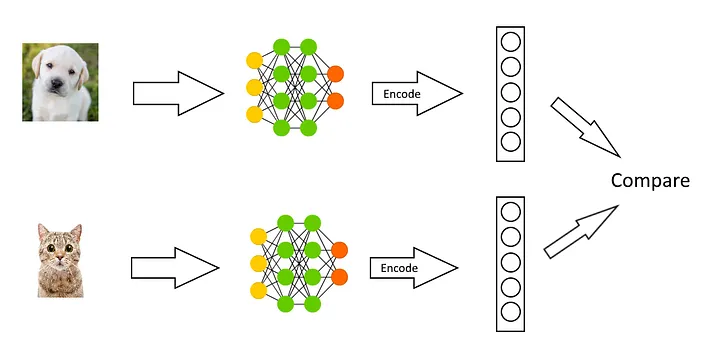
\includegraphics[width=\linewidth]{Parallel.png}
	\caption{The basic structure of a Siamese Neural Network, illustrating its parallel nature. Source: \autocite{craeymeersch}.}
	\label{fig:parallel}
\end{figure}

The key difference can be found with "learning\_size" in the tensor shape of "images", where "learning\_size" represents the number of images being used in parallel for the learning process as seen in (Figure \ref{fig:parallel}). For example, it would makes sense for a triplet loss similarity learning architecture, the learning\_size would be 3, as there are 3 images being used in parallel for the learning process. However, this variable allows for other architectures to be supported as well. 

\begin{figure} % Single column figure
	
\includegraphics[width=\linewidth]{Triplet.png}
	\caption{An illustration of triplet loss for SiNNs, resulting in a "learning\_size" = 2. Source: \autocite{craeymeersch}.}
	\label{fig:triplet}
\end{figure}

Additionally, "labels" is changed to a different shape to also allow for other architectures to be supported. For example, if the architecture is a triplet loss similarity learning architecture, the labels would be of shape (batch\_size, 2), where the first column represents the similarity of the first image (the anchor) to the second image, and the second column represents the similarity of the first image (the anchor) to the third image. Meanwhile in a case where the learning\_size is 2, the labels would be of shape (batch\_size, 1), where the first column represents the similarity of the first image (the anchor) to the second image.

\section{Initial Approaches}

\subsection{Permutation Approach}
The initial attempt towards tackling this challenge was anchored in the idea of iterating through the directory, and producing every possible combination of images, this is accomplished by the code in Figure \ref{fig:initial}.

\begin{figure*} % Single column figure
	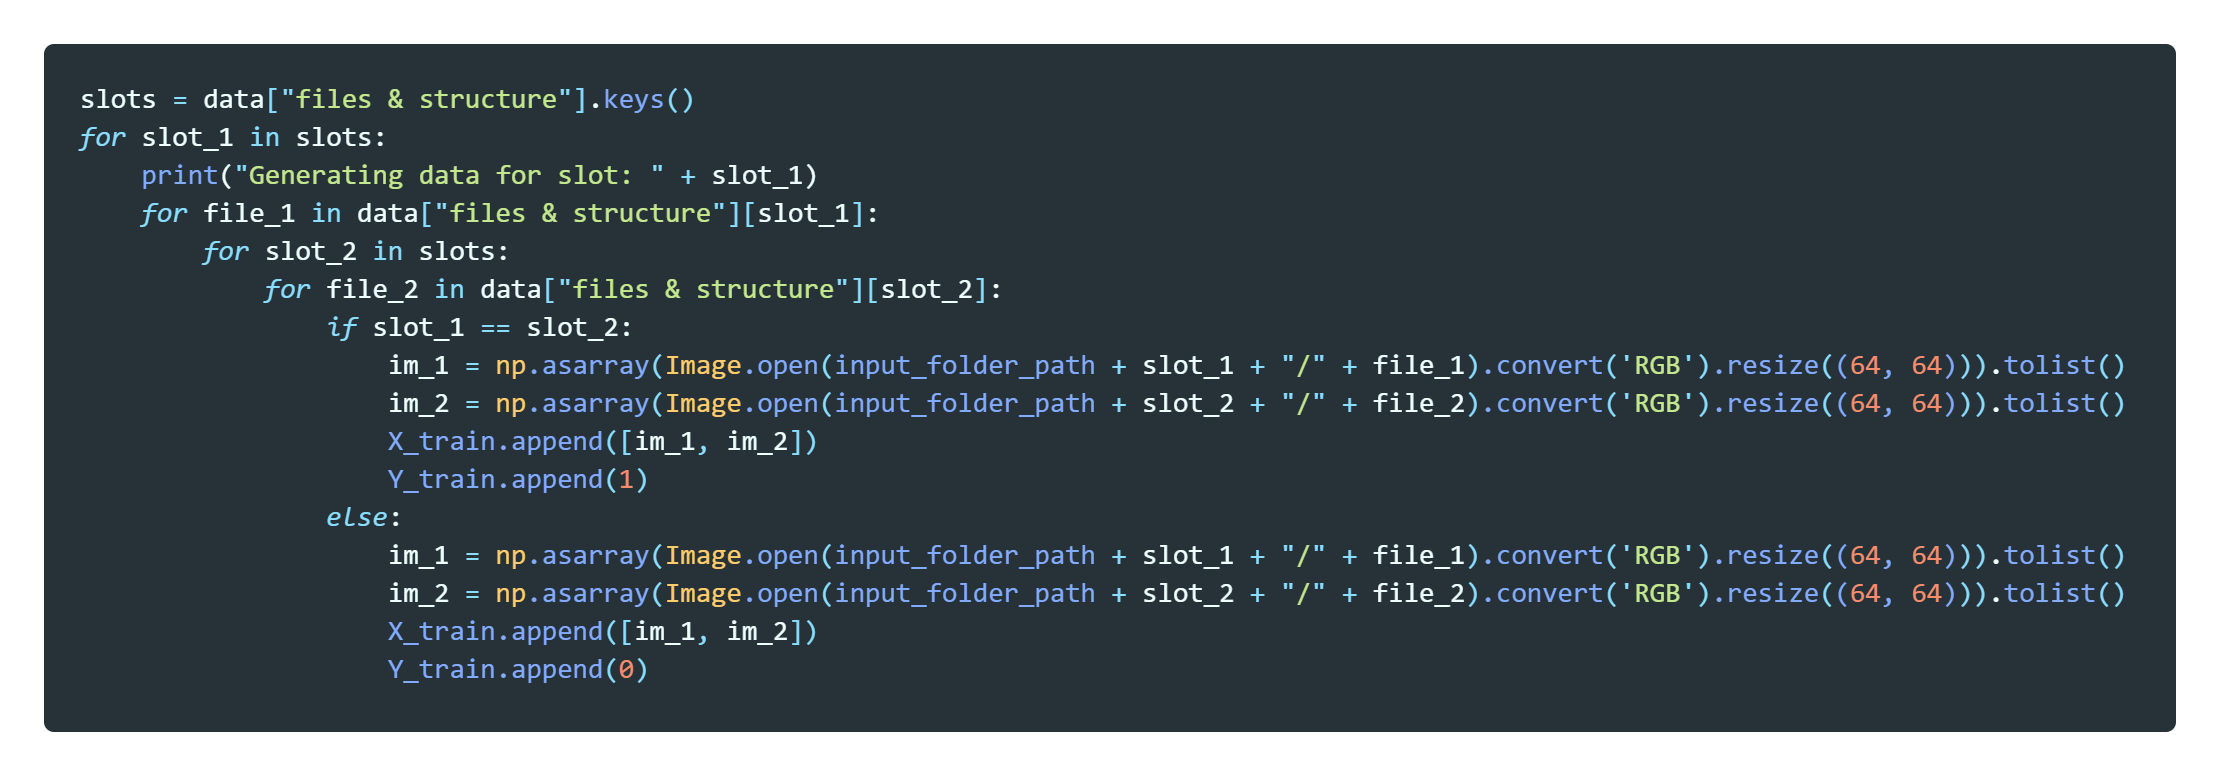
\includegraphics[width=\linewidth]{initial.png}
	\caption{The initial Python code for developing a generator for Siamese Neural Networks.}
	\label{fig:initial}
\end{figure*}

The approach illustrated in Figure \ref{fig:initial} is a permutation approach, where the generator would iterate through the directory, and produce every possible combination of images. For example, if the directory had 10 images of class 0, 10 images of class 1, and 10 images of class 2 the generator would produce the following combinations:
% TODO


However, this approach is not scalable. % as it would require the entire dataset to be loaded into memory, and would in turn be very slow. % This is because the generator would have to iterate through the entire dataset for every batch, and would have to produce every possible combination of images for every batch. % This is not a viable solution, and thus a different approach was needed.

Firstly, this approach will lead to data heavily biased towards dissimilar images due to the nature of permutations. For example, look at a directory database that follows the structure shown in Table \ref{tab:structure}.

\begin{table}[h!] % Single column table
	\caption{Example structure of a tree directory dataset.}
	\centering
	\begin{tabular}{l l r}
		\toprule
		\multicolumn{2}{c}{Class} \\
		\cmidrule(r){1-2}
		Number (n) & Identification & Data Count (n[l]) \\
		\midrule
		0 & Red Oak & 10 \\
		1 & Cedar & 10 \\
		2 & Dogwood & 10 \\
		3 & Maple & 10 \\
		4 & Hickory & 10 \\
		\bottomrule
	\end{tabular}
	\label{tab:structure}
\end{table}

Assuming that within the main directory we see 5 folders representing classes, each with 10 images; With a Tuplet loss, and using 1 singular image of a class as an anchor, we can see that there may only be 10 possible positive cases (including pairing the anchor with itself), and 40 possible negative cases. Of course, as we traverse across the dataset we will acquire additional positive cases, however, the issue of misrepresentation of the dataset is only exacerbated.  
% and that we are using a triplet loss architecture, the generator would produce 10,000 batches, where each batch would contain 3 images, and 2 labels. However, the generator would produce 10,000 batches of 3 images, where 2 of the images are from the same class, and 1 image is from a different class. This is because the generator would produce every possible combination of images, and would not take into account the class of the images. This would lead to the model being trained on a lot of dissimilar images, and would not be a good representation of the dataset.

The formulas for finding such values for one anchor image may be seen below (it should be noted that the (\#\_of\_positives) includes the anchor image being compared to itself):

\[ \alpha = (anchor\_class\_length) \]
\[ \sum_{n = 0}^4 n[l] - \alpha = (\#\_of\_negatives) \]
\[ \alpha = (\#\_of\_positives) \]

Extending this logic, it is also possible to determine these same values when traversing across the entire dataset (AKA the total positive and negative cases or pairs):

\[ \sum_{n = 0}^4 n[l] - \alpha = (\#\_of\_negatives) \]
\[ \sum_{n = 0}^4 n[l] - \alpha = (\#\_of\_unique\_negatives) \]
\[ \alpha = (\#\_of\_positives) \]
\[ \alpha-1 = (\#\_of\_unique\_positives) \]

%X 123
%Y 123
%Z 123
% x1, x1 p
% x1, x2 p
% x1, x3 p
% x1, y1 n
% x1, y2 n
% x1, y3 n
% x1, z1 n
% x1, z2 n
% x1, z3 n

% x2, x1 p
% x2, x2 p
% x2, x3 p
% x2, y1 n
% x2, y2 n
% x2, y3 n
% x2, z1 n
% x2, z2 n
% x2, z3 n

% x3, x1 p
% x3, x2 p
% x3, x3 p
% x3, y1 n
% x3, y2 n
% x3, y3 n
% x3, z1 n
% x3, z2 n
% x3, z3 n

% y1, x1 n
% y1, x2 n
% y1, x3 n
% y1, y1 p
% y1, y2 p
% y1, y3 p
% y1, z1 n
% y1, z2 n
% y1, z3 n

% y2, x1 n
% y2, x2 n
% y2, x3 n
% y2, y1 p
% y2, y2 p
% y2, y3 p
% y2, z1 n
% y2, z2 n
% y2, z3 n

% y3, x1 n
% y3, x2 n
% y3, x3 n
% y3, y1 p
% y3, y2 p
% y3, y3 p
% y3, z1 n
% y3, z2 n
% y3, z3 n

% z1, x1 n
% z1, x2 n
% z1, x3 n
% z1, y1 n
% z1, y2 n
% z1, y3 n
% z1, z1 p
% z1, z2 p
% z1, z3 p

% z2, x1 n
% z2, x2 n
% z2, x3 n
% z2, y1 n
% z2, y2 n
% z2, y3 n
% z2, z1 p
% z2, z2 p
% z2, z3 p

% z3, x1 n
% z3, x2 n
% z3, x3 n
% z3, y1 n
% z3, y2 n
% z3, y3 n
% z3, z1 p
% z3, z2 p
% z3, z3 p



% TODO

% AKA a general solution to this being ___

Additionally, in the case of smaller datasets, it will lead to a lot of unnecessary loops, especially, if we are interested in getting a unique pair of images, and not one the model has already seen.

% It also doesn't yield sequentially
% Not random, it doesn't support randomization

The reason uniqueness of a pair is important is because if we are interested in training a Siamese Neural Network, we want to ensure that the model is not trained on the same pair of images, as this would lead to the model overfitting to the dataset, and would not be able to generalize well to new data.

So how can we ensure uniqueness? Through a combination approach, this is possible.

Finally, this method doesn't match our requirements, nor does it yield data sequentially, it produces 2 datasets, one being x\_train, and the other being y\_train.

\subsection{Combination Approach}

Using combinations as opposed to permutations allows for uniqueness, because order doesn't matter in the case of siamese neural networks

% Mauris interdum porttitor fringilla. Proin tincidunt sodales leo at ornare. Donec tempus magna non mauris gravida luctus. Cras vitae arcu vitae mauris eleifend scelerisque. Nam sem sapien, vulputate nec felis eu, blandit convallis risus. Pellentesque sollicitudin venenatis tincidunt. In et ipsum libero. Nullam tempor ligula a massa convallis pellentesque. Mauris interdum porttitor fringilla. Proin tincidunt sodales leo at ornare. Donec tempus magna non mauris gravida luctus. Cras vitae arcu vitae mauris eleifend scelerisque. Nam sem sapien, vulputate nec felis eu, blandit convallis risus. Pellentesque sollicitudin venenatis tincidunt. In et ipsum libero. Nullam tempor ligula a massa convallis pellentesque.
% 
% %------------------------------------------------
% 
% \section{Results}
% 
% Referencing a table using its label: Table \ref{tab:distcounts}.
% 
% \begin{table*} % Full width table (notice the starred environment)
% 	\caption{Example two column table with fixed-width columns.}
% 	\centering % Horizontally center the table
% 	\begin{tabular}{L{0.2\linewidth} L{0.2\linewidth} R{0.15\linewidth}} % Manually specify column alignments with L{}, R{} or C{} and widths as a fixed amount, usually as a proportion of \linewidth
% 		\toprule
% 		\multicolumn{2}{c}{Location} \\
% 		\cmidrule(r){1-2}
% 		East Distance & West Distance & Count \\
% 		\midrule
% 		100km & 200km & 422 \\
% 		350km & 1000km & 1833 \\
% 		600km & 1200km & 890 \\
% 		\bottomrule
% 	\end{tabular}
% \end{table*}
% 
% Aenean feugiat pellentesque venenatis. Sed faucibus tristique tortor vel ultrices. Donec consequat tellus sapien. Nam bibendum urna mauris, eget sagittis justo gravida vel. Mauris nisi lacus, malesuada sit amet neque ut, venenatis tempor orci. Curabitur feugiat sagittis molestie. Duis euismod arcu vitae quam scelerisque facilisis. Praesent volutpat eleifend tortor, in malesuada dui egestas id. Donec finibus ac risus sed pellentesque. Donec malesuada non magna nec feugiat. Mauris eget nibh nec orci congue porttitor vitae eu erat. Sed commodo ipsum ipsum, in elementum neque gravida euismod. Cras mi lacus, pulvinar ut sapien ut, rutrum sagittis dui. Donec non est a metus varius finibus. Pellentesque rutrum pellentesque ligula, vitae accumsan nulla hendrerit ut.
% 
% \begin{figure} % Single column figure
% 	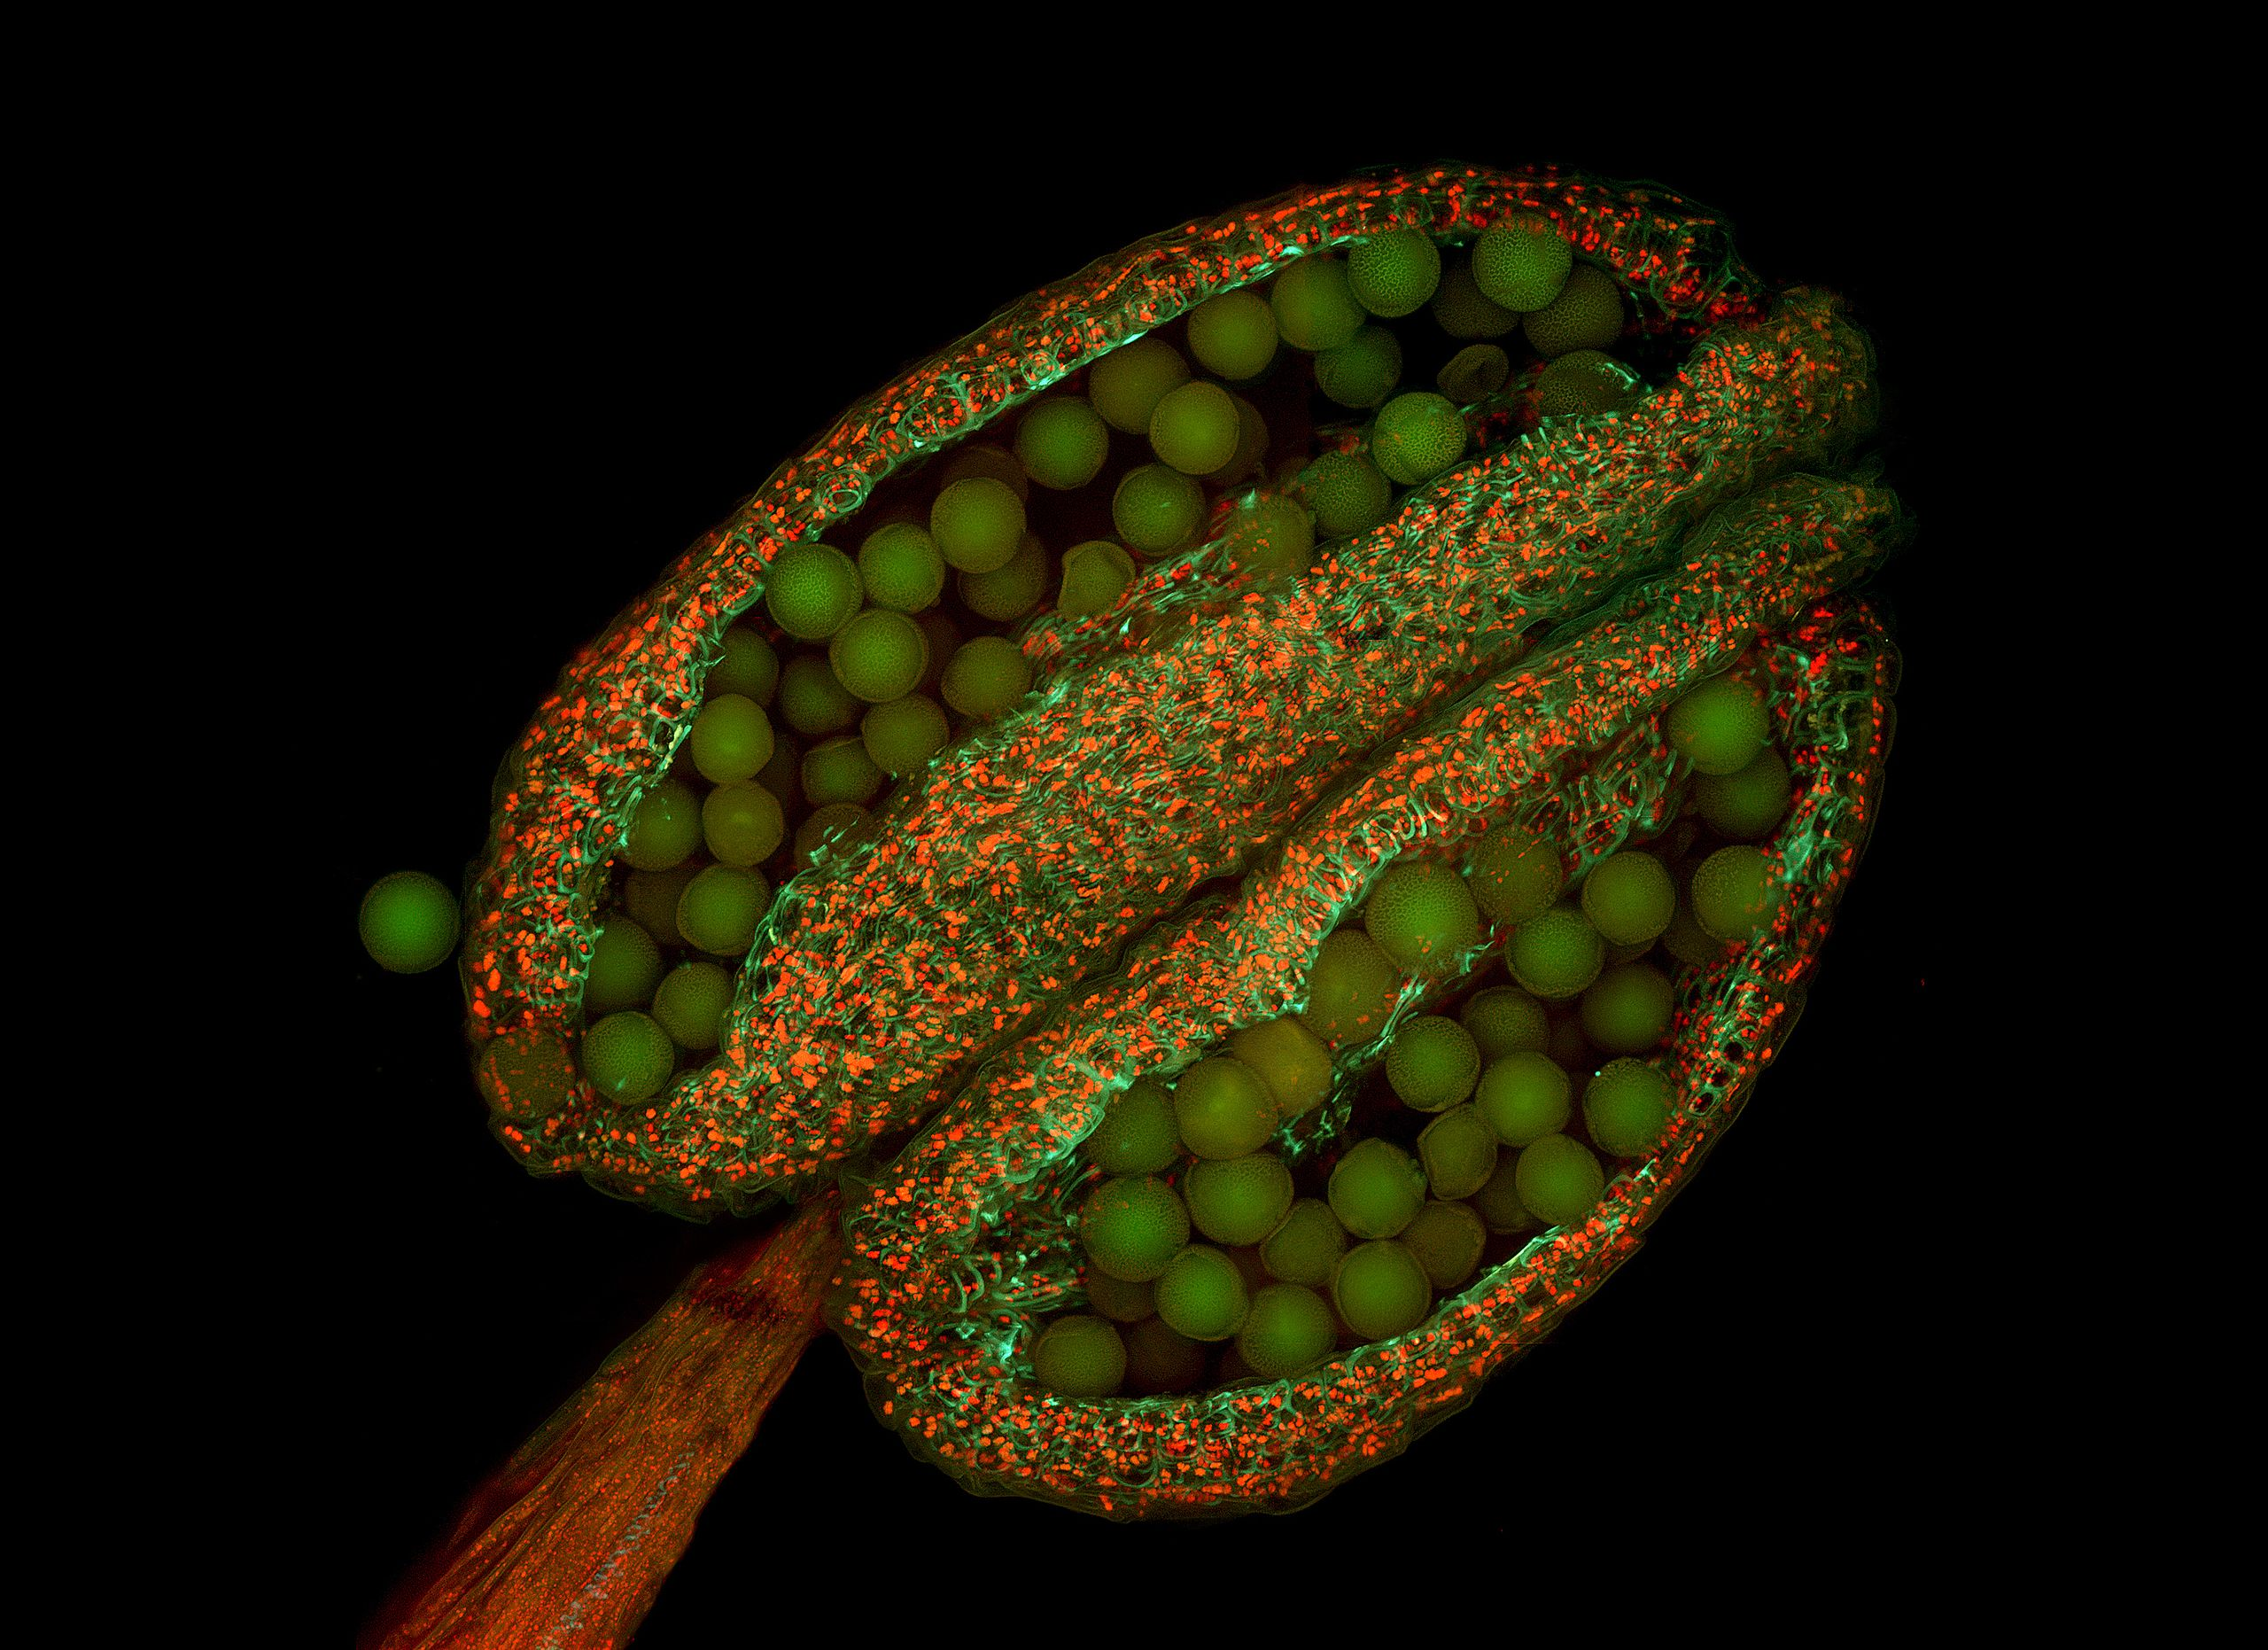
\includegraphics[width=\linewidth]{Tolmukapea.jpg}
% 	\caption{Anther of thale cress (Arabidopsis thaliana), fluorescence micrograph. Source: Heiti Paves, \href{https://commons.wikimedia.org/wiki/File:Tolmukapea.jpg}{https://commons.wiki-\\media.org/wiki/File:Tolmukapea.jpg}.}
% 	\label{fig:tcanther}
% \end{figure}
% 
% Referencing a figure using its label: Figure \ref{fig:tcanther}.
% 
% Aenean porttitor eros non pharetra congue. Proin in odio in dolor luctus auctor ac et mi. Etiam euismod mi sed lectus fringilla pretium. Phasellus tristique maximus lectus et sodales. Mauris feugiat ligula quis semper luctus. Nam sit amet felis sed leo fermentum aliquet. Mauris arcu dui, posuere id sem eget, cursus pulvinar mi. Donec nec lacus non lectus fermentum scelerisque et at nibh. Sed tristique, metus ac vestibulum porta, tortor lectus placerat lorem, et convallis tellus dolor eget ante. Pellentesque dui ligula, hendrerit a purus et, volutpat tempor lectus. Mauris nec purus nec mauris rhoncus pellentesque. Quisque quis diam sed est lacinia congue. Donec magna est, hendrerit sed metus vel, accumsan rutrum nibh.
% 
% \begin{figure*} % Two column figure (notice the starred environment)
% 	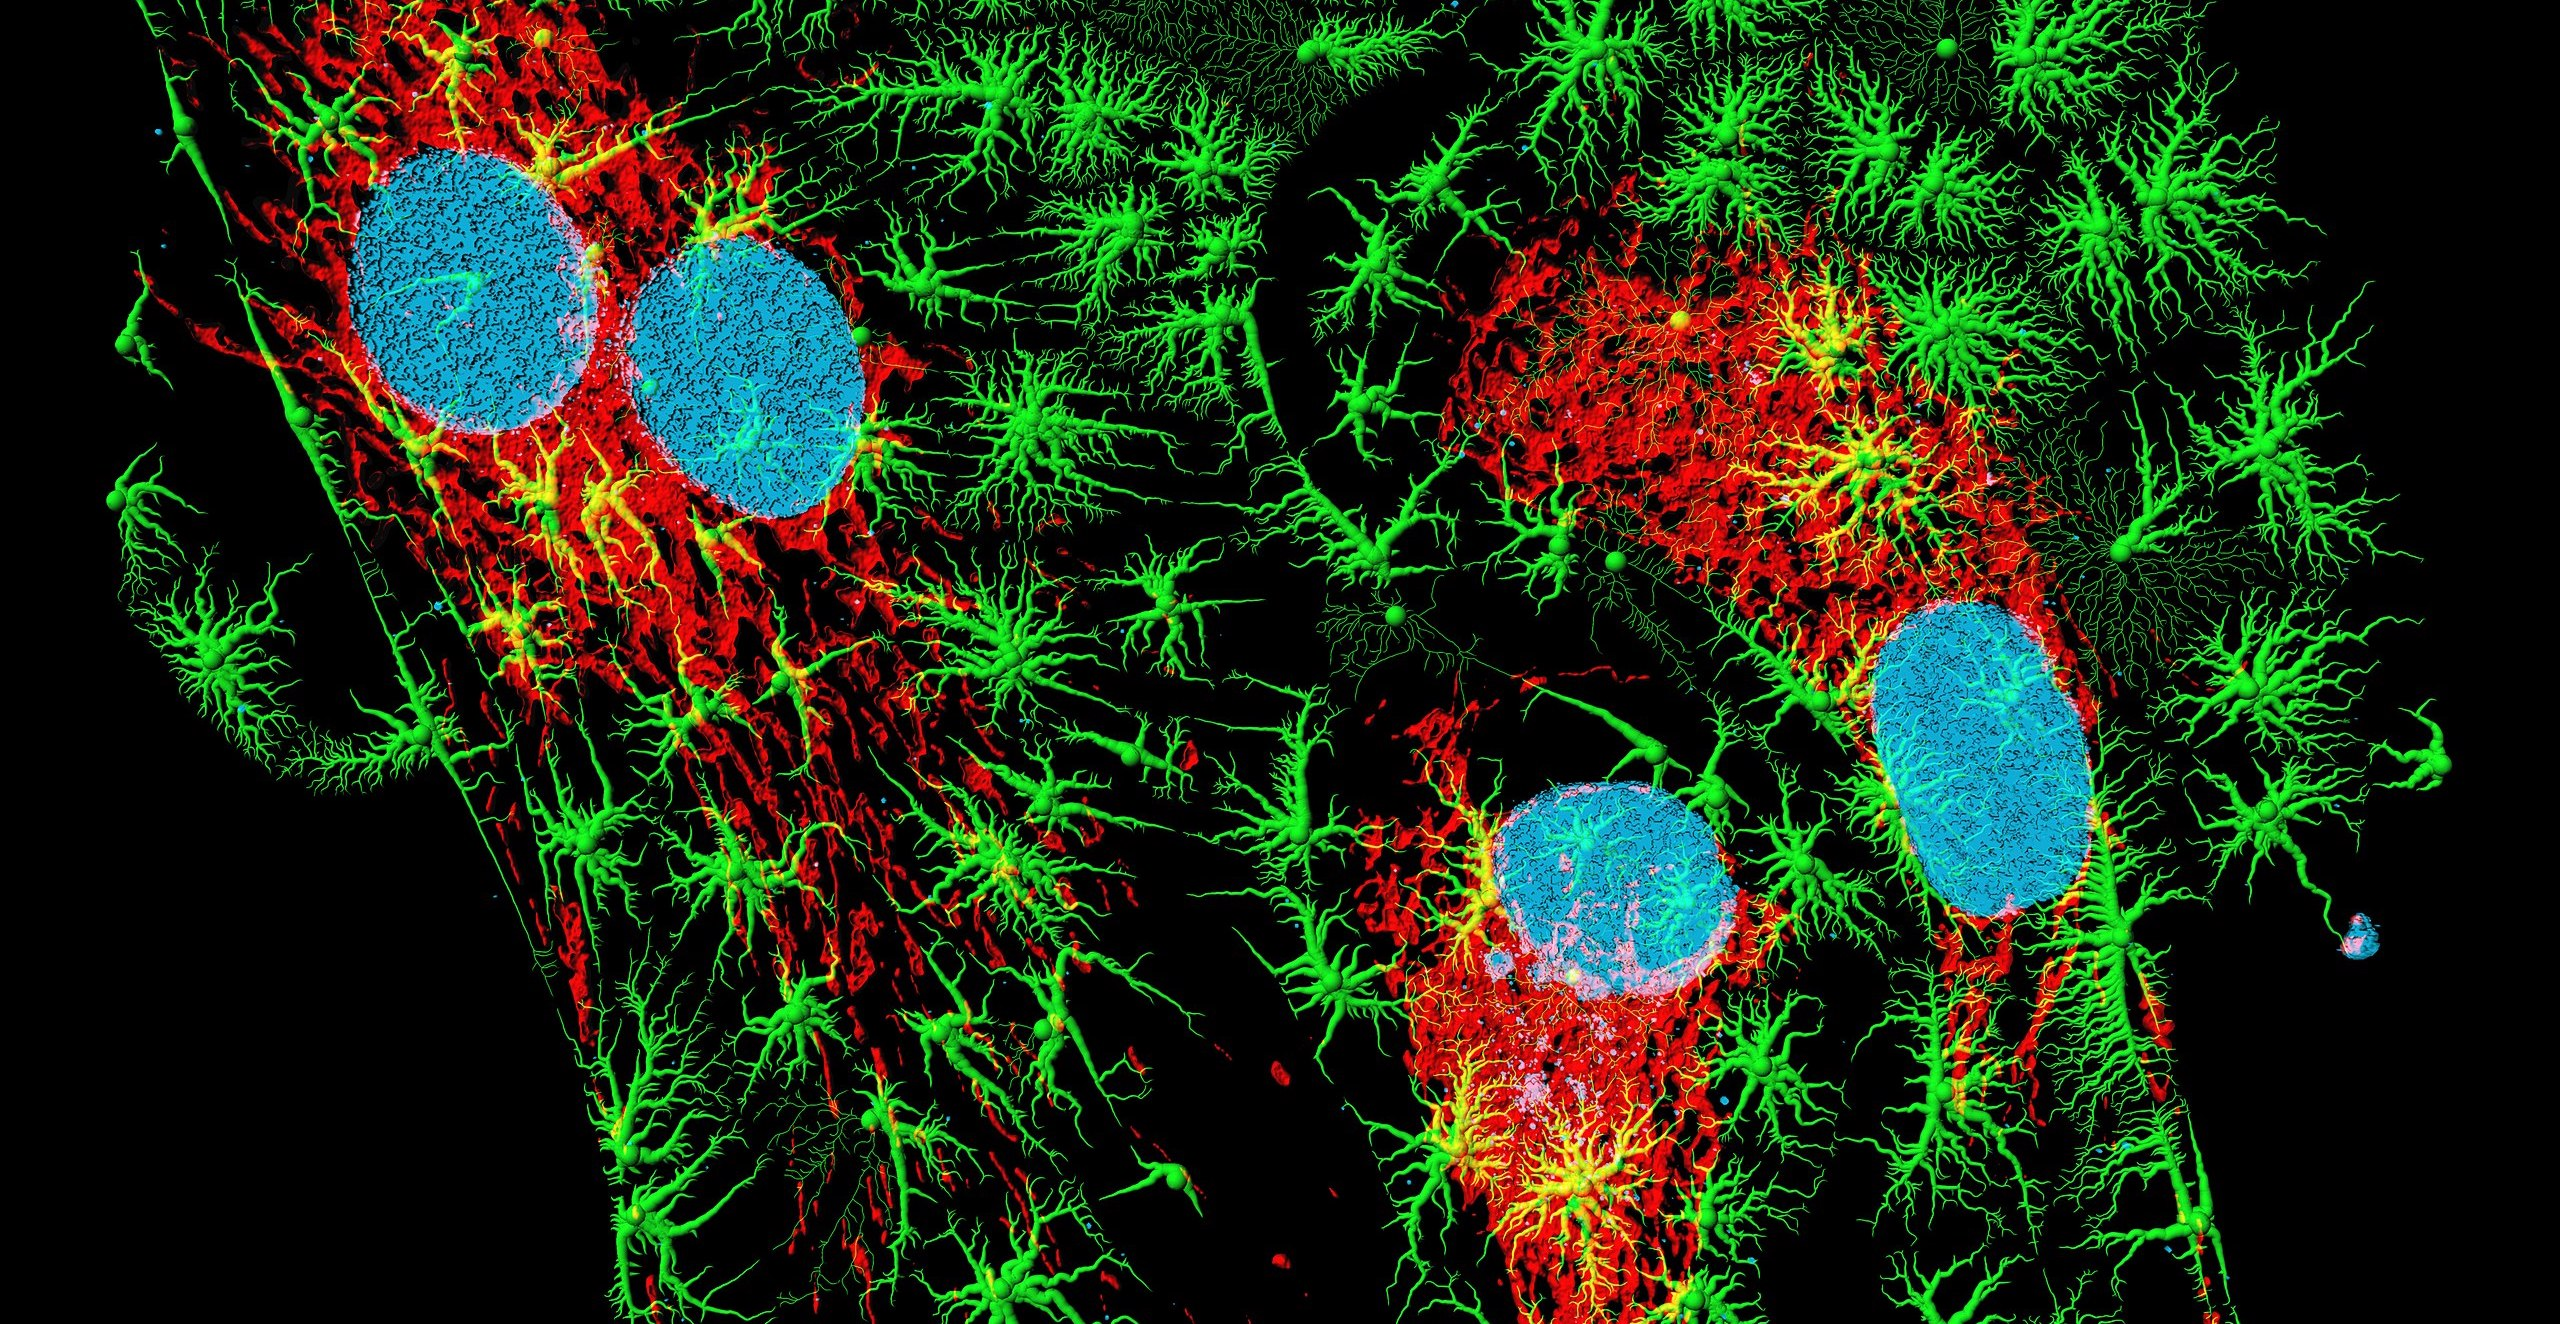
\includegraphics[width=\linewidth]{Fibroblastid.jpg}
% 	\caption{Bovine pulmonary artery endothelial cells in culture. Blue: nuclei; red: mitochondria; green: microfilaments. Computer generated image from a 3D model based on a confocal laser scanning microscopy using fluorescent marker dyes. Source: Heiti Paves, \href{https://commons.wikimedia.org/wiki/File:Fibroblastid.jpg}{https://commons.wikimedia.org/wiki/File:Fibroblastid.jpg}.}
% 	\label{fig:bpartery}
% \end{figure*}
% 
% Orci varius natoque penatibus et magnis dis parturient montes, nascetur ridiculus mus. Etiam cursus lectus purus, tempus iaculis quam dictum tristique. Nam interdum sapien nec tempor mattis. Quisque id sapien nisi. Mauris vehicula ornare eros vel efficitur. Nulla consectetur, turpis quis fringilla tincidunt, mi neque iaculis lectus, vel commodo elit odio non ex. Duis facilisis, purus ac viverra iaculis, turpis lectus ultrices ante, ac vestibulum ligula magna in libero. Etiam tristique maximus lacinia. Vestibulum hendrerit, lacus malesuada laoreet blandit, sapien velit sollicitudin nunc, eu porttitor urna ligula at lorem. Aliquam faucibus eros in fermentum venenatis. Fusce consectetur congue pellentesque. Suspendisse at nisi sit amet est porttitor cursus. Cras placerat faucibus nunc, a laoreet justo dignissim sit amet.
% 
% \subsection{International Support}
% 
% \noindent àáâäãåèéêëìíîïòóôöõøùúûüÿýñçčšž
% 
% \noindent ÀÁÂÄÃÅÈÉÊËÌÍÎÏÒÓÔÖÕØÙÚÛÜŸÝÑ
% 
% \noindent ßÇŒÆČŠŽ
% 
% \subsection{Links}
% 
% This is a clickable URL link: \href{https://www.latextemplates.com}{LaTeX Templates}. This is a clickable email link: \href{mailto:vel@latextemplates.com}{vel@latextemplates.com}. This is a clickable monospaced URL link: \url{https://www.LaTeXTemplates.com}.
% 
% %------------------------------------------------
% 
% \section{Discussion}
% 
% This statement requires citation \autocite{Smith:2023qr}. This statement requires multiple citations \autocite{Smith:2023qr, Smith:2024jd}. This statement contains an in-text citation, for directly referring to a citation like so: \textcite{Smith:2024jd}.
% 
% \subsection{Subsection One}
% 
% Suspendisse potenti. Vivamus suscipit dapibus metus. Proin auctor iaculis ex, id fermentum lectus dapibus tristique. Nullam maximus eros eget leo pretium dapibus. Nunc in auctor erat, id interdum risus. Suspendisse aliquet vehicula accumsan. In vestibulum efficitur dictum. Sed ultrices, libero nec fringilla feugiat, elit massa auctor ligula, vehicula tempor ligula felis in lectus. Suspendisse sem dui, pharetra ut sodales eu, suscipit sit amet felis. Donec pretium viverra ante, ac pulvinar eros. Suspendisse gravida consectetur urna. Pellentesque vitae leo porta, imperdiet eros eget, posuere sem. Praesent eget leo efficitur odio bibendum condimentum sit amet vel ex. Nunc maximus quam orci, quis pulvinar nibh eleifend ac. Quisque consequat lacus magna, eu posuere tellus iaculis ac. Sed vitae tortor tincidunt ante sagittis iaculis.
% 
% \subsection{Subsection Two}
% 
% Nullam mollis tellus lorem, sed congue ipsum euismod a. Donec pulvinar neque sed ligula ornare sodales. Nulla sagittis vel lectus nec laoreet. Nulla volutpat malesuada turpis at ultricies. Ut luctus velit odio, sagittis volutpat erat aliquet vel. Donec ac neque eget neque volutpat mollis. Vestibulum viverra ligula et sapien bibendum, vel vulputate ex euismod. Curabitur nec velit velit. Aliquam vulputate lorem elit, id tempus nisl finibus sit amet. Curabitur ex turpis, consequat at lectus id, imperdiet molestie augue. Curabitur eu eros molestie purus commodo hendrerit. Quisque auctor ipsum nec mauris malesuada, non fringilla nibh viverra. Quisque gravida, metus quis semper pulvinar, dolor nisl suscipit leo, vestibulum volutpat ante justo ultrices diam. Sed id facilisis turpis, et aliquet eros.
% 
% \subsubsection{Subsubsection Example}
% 
% Duis venenatis eget lectus a aliquet. Integer vulputate ante suscipit felis feugiat rutrum. Aliquam eget dolor eu augue elementum ornare. Nulla fringilla interdum volutpat. Sed tincidunt, neque quis imperdiet hendrerit, turpis sapien ornare justo, ac blandit felis sem quis diam. Proin luctus urna sit amet felis tincidunt, sed congue nunc pellentesque. Ut faucibus a magna faucibus finibus. Etiam id mi euismod, auctor nisi eget, pretium metus. Proin tincidunt interdum mi non interdum. Donec semper luctus dolor at elementum. Aenean eu congue tortor, sed hendrerit magna. Quisque a dolor ante. Mauris semper id urna id gravida. Vestibulum mi tortor, finibus eu felis in, vehicula aliquam mi.
% 
% Aliquam arcu turpis, ultrices sed luctus ac, vehicula id metus. Morbi eu feugiat velit, et tempus augue. Proin ac mattis tortor. Donec tincidunt, ante rhoncus luctus semper, arcu lorem lobortis justo, nec convallis ante quam quis lectus. Aenean tincidunt sodales massa, et hendrerit tellus mattis ac. Sed non pretium nibh. 
% 
% Donec cursus maximus luctus. Vivamus lobortis eros et massa porta porttitor. Nam vitae suscipit mi. Pellentesque ex tellus, iaculis vel libero at, cursus pretium sapien. Curabitur accumsan velit sit amet nulla lobortis, ut pretium ex aliquam. Proin eget volutpat orci. Morbi eu aliquet turpis. Vivamus molestie urna quis tempor tristique. Proin hendrerit sem nec tempor sollicitudin.
% 
%----------------------------------------------------------------------------------------
%	 REFERENCES
%----------------------------------------------------------------------------------------

\printbibliography % Output the bibliography

%----------------------------------------------------------------------------------------

\end{document}
